% Author: Seongjin Lee 
% Gyeongsang National University, Korea 
% 
% 2021-02-26
%

\documentclass[newPxFont,sthlmFooter,nooffset]{beamer}
\usepackage{kotex}
%\usetheme{sthlm}
\usepackage{../style/beamerthemesthlm}
\hypersetup{pdfauthor={Seongjin Lee (insight@gnu.ac.kr)},
            pdfsubject={Data Structure and Algorithm, Lecture Note},
            pdfkeywords={Data Structure, Algorithm, Lecture, Note},
            pdfmoddate={D: \pdfdate},
            pdfcreator={Seongjin Lee}}

%\setbeamertemplate{footline}[text line]{%
%    \parbox{\linewidth}{\vspace*{-8pt} \insertsectionhead  \hfill\insertshortauthor\hfill\insertpagenumber}}
%\setbeamertemplate{navigation symbols}{}

\usepackage{tkz-graph}

\setbeamertemplate{blocks}[rounded]

\title{Data Structure and Algorithm}
\subtitle{Class 9}
\author[SJL]{Seongjin Lee}
\institute{\href{mailto:insight@gnu.ac.kr}{insight@gnu.ac.kr}\\\url{http://resourceful.github.io}\\Systems Research Lab.\\GNU}
\date{2021-02-26} 

\begin{document}



\frame[plain,t]{\titlepage} 

\frame{\frametitle{Table of contents}\tableofcontents} 


%---------------------------------------------------------
\section{Graph Operations}


\begin{frame}[t]
  \frametitle{Some of the Graph Problems are}
  \begin{itemize}
  \item Path Finding
  \item Connectedness
  \item Spanning tree
  \end{itemize}


\end{frame}





\subsection{Path Finding}
\begin{frame}[t]
  \frametitle{Path Finding}
  \begin{itemize}
  \item Path length between 1 and 8
  \end{itemize}

  \begin{center}
    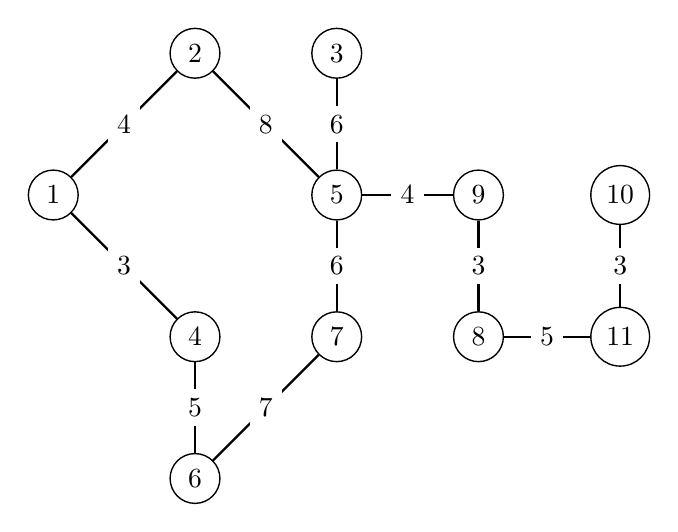
\begin{tikzpicture}
    \GraphInit[vstyle=Normal]\SetGraphUnit{1.8}
    \Vertex{1}
    \NOEA(1){2}
    \SOEA(2){5}
    \NO(5){3}
    \SOEA(1){4}
    \SO(4){6}
    \NOEA(6){7}
    \EA(5){9}
    \SO(9){8}
    \SOEA(9){11}
    \EA(9){10}
    \Edges[label=6](5, 3)
    \Edges[label=3](1, 4)
    \Edges[label=5](4, 6)
    \Edges[label=7](6, 7)
    \Edges[label=6](7, 5)
    \Edges[label=5](8, 11)
    \Edges[label=3](11, 10)
    \Edges[label=4](1, 2)
    \Edges[label=8](2, 5)
    \Edges[label=4](5, 9)
    \Edges[label=3](8, 9)
    \end{tikzpicture}
  \end{center}

\end{frame}

\begin{frame}[t]
  \frametitle{Path Finding}
  \begin{itemize}
  \item Edges (1, 2), (2, 5), (5, 9), and (9, 8) length = 19
  \end{itemize}

  \begin{center}
    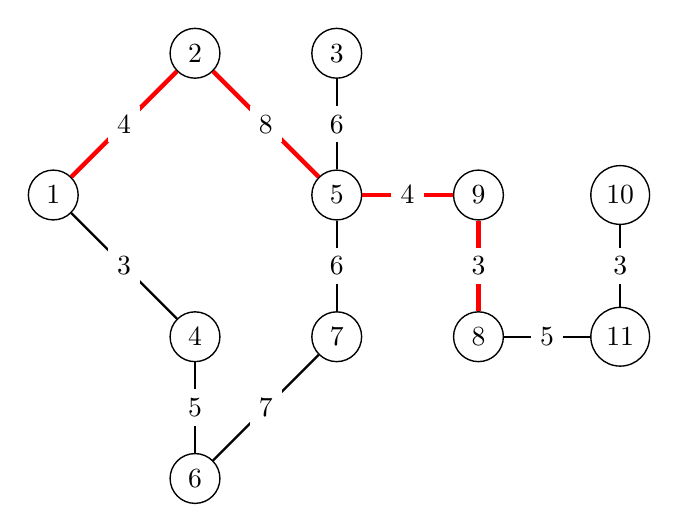
\begin{tikzpicture}
    \GraphInit[vstyle=Normal]\SetGraphUnit{1.8}
    \Vertex{1}
    \NOEA(1){2}
    \SOEA(2){5}
    \NO(5){3}
    \SOEA(1){4}
    \SO(4){6}
    \NOEA(6){7}
    \EA(5){9}
    \SO(9){8}
    \SOEA(9){11}
    \EA(9){10}
    \Edges[label=6](5, 3)
    \Edges[label=3](1, 4)
    \Edges[label=5](4, 6)
    \Edges[label=7](6, 7)
    \Edges[label=6](7, 5)
    \Edges[label=5](8, 11)
    \Edges[label=3](11, 10)

    \SetUpEdge[style={ultra thick}, color=red]
    \Edges[label=4](1, 2)
    \Edges[label=8](2, 5)
    \Edges[label=4](5, 9)
    \Edges[label=3](8, 9)
    \end{tikzpicture}
  \end{center}

\end{frame}

\begin{frame}[t]
  \frametitle{Path Finding}
  \begin{itemize}
  \item Edges (1, 4), (4, 6), (6, 7), (5, 9) and (9, 8) length = 28
  \end{itemize}

  \begin{center}
    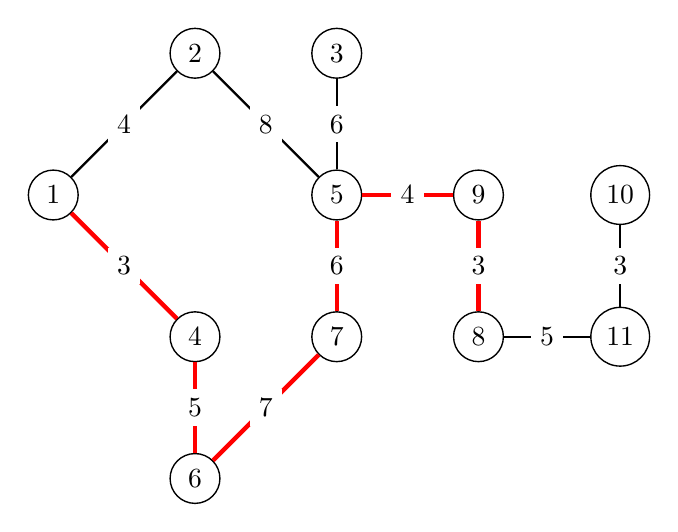
\begin{tikzpicture}
    \GraphInit[vstyle=Normal]\SetGraphUnit{1.8}
    \Vertex{1}
    \NOEA(1){2}
    \SOEA(2){5}
    \NO(5){3}
    \SOEA(1){4}
    \SO(4){6}
    \NOEA(6){7}
    \EA(5){9}
    \SO(9){8}
    \SOEA(9){11}
    \EA(9){10}
    \Edges[label=6](5, 3)
    \Edges[label=5](8, 11)
    \Edges[label=3](11, 10)
    \Edges[label=4](1, 2)
    \Edges[label=8](2, 5)

    \SetUpEdge[style={ultra thick}, color=red]
    \Edges[label=3](1, 4)
    \Edges[label=5](4, 6)
    \Edges[label=7](6, 7)
    \Edges[label=6](7, 5)
    \Edges[label=4](5, 9)
    \Edges[label=3](8, 9)
    \end{tikzpicture}
  \end{center}

\end{frame}


\begin{frame}[t]
  \frametitle{Example of No Path}
  \begin{itemize}
  \item No path between 4 to 11
  \end{itemize}
  \begin{center}
    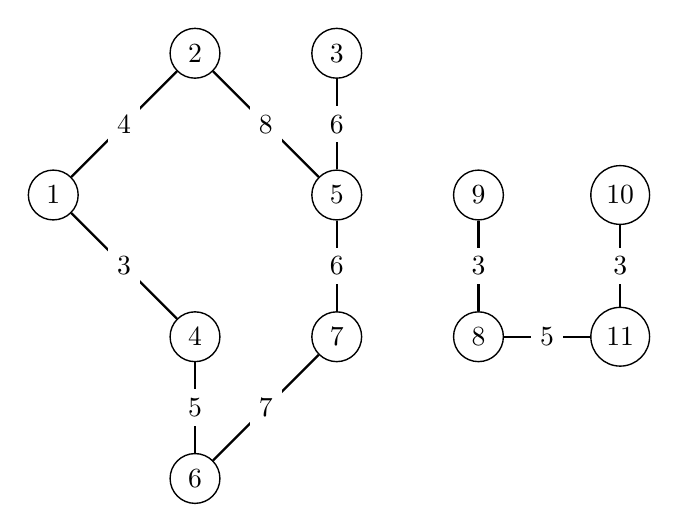
\begin{tikzpicture}
    \GraphInit[vstyle=Normal]\SetGraphUnit{1.8}
    \Vertex{1}
    \NOEA(1){2}
    \SOEA(2){5}
    \NO(5){3}
    \SOEA(1){4}
    \SO(4){6}
    \NOEA(6){7}
    \EA(5){9}
    \SO(9){8}
    \SOEA(9){11}
    \EA(9){10}
    \Edges[label=6](5, 3)
    \Edges[label=5](8, 11)
    \Edges[label=3](11, 10)
    \Edges[label=4](1, 2)
    \Edges[label=8](2, 5)
    \Edges[label=3](1, 4)
    \Edges[label=5](4, 6)
    \Edges[label=7](6, 7)
    \Edges[label=6](7, 5)
    \Edges[label=3](8, 9)
    \end{tikzpicture}
  \end{center}

\end{frame}







\subsection{Connected Graph}
\begin{frame}[t]
  \frametitle{Connected Graph}
  \begin{itemize}
  \item Undirected graph
  \item There is a path between every pair of vertices
  \end{itemize}
\bigskip
\begin{itemize}
\item A directed graph $G=(V, E)$ is \textbf{strongly connected} if, for every pair of vertices $u, v$ in $V$, there is a directed path from $u$ to $v$ and also from $v$ to $u$
\end{itemize}

\begin{columns}
  \begin{column}{0.4\textwidth}
    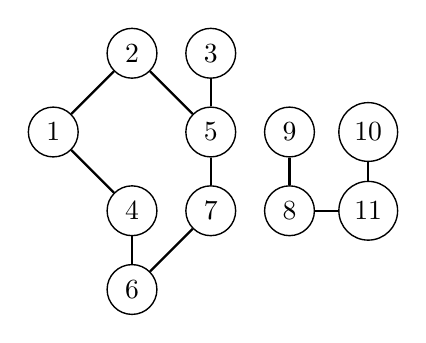
\begin{tikzpicture}
    \GraphInit[vstyle=Normal]\SetGraphUnit{1}
    \Vertex{1}
    \NOEA(1){2}
    \SOEA(2){5}
    \NO(5){3}
    \SOEA(1){4}
    \SO(4){6}
    \NOEA(6){7}
    \EA(5){9}
    \SO(9){8}
    \SOEA(9){11}
    \EA(9){10}
    \Edges(5, 3)
    \Edges(8, 11)
    \Edges(11, 10)
    \Edges(1, 2)
    \Edges(2, 5)
    \Edges(1, 4)
    \Edges(4, 6)
    \Edges(6, 7)
    \Edges(7, 5)
    \Edges(8, 9)
    \end{tikzpicture}
      
Not connected graph
  \end{column}
  \begin{column}{0.4\textwidth}
    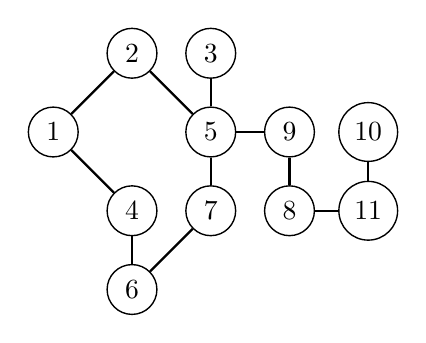
\begin{tikzpicture}
    \GraphInit[vstyle=Normal]\SetGraphUnit{1}
    \Vertex{1}
    \NOEA(1){2}
    \SOEA(2){5}
    \NO(5){3}
    \SOEA(1){4}
    \SO(4){6}
    \NOEA(6){7}
    \EA(5){9}
    \SO(9){8}
    \SOEA(9){11}
    \EA(9){10}
    \Edges(5, 3)
    \Edges(8, 11)
    \Edges(11, 10)
    \Edges(1, 2)
    \Edges(2, 5)
    \Edges(1, 4)
    \Edges(4, 6)
    \Edges(6, 7)
    \Edges(7, 5)
    \Edges(8, 9)
    \Edges(5, 9)
    \end{tikzpicture}

Connected Graph      
  \end{column}
\end{columns}
\end{frame}


\begin{frame}[t]
  \frametitle{Connected Components}

\begin{center}
    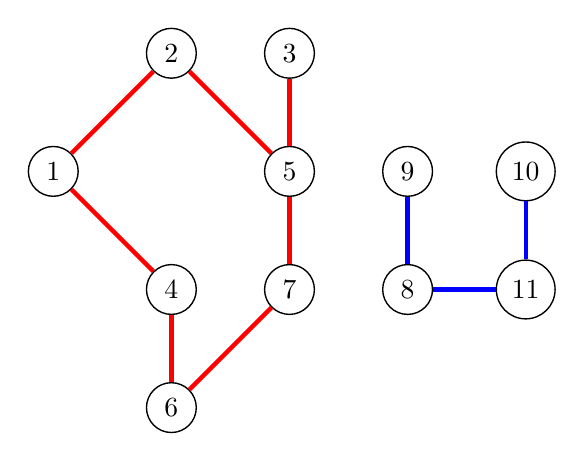
\begin{tikzpicture}
    \GraphInit[vstyle=Normal]\SetGraphUnit{1.5}
    \Vertex{1}
    \NOEA(1){2}
    \SOEA(2){5}
    \NO(5){3}
    \SOEA(1){4}
    \SO(4){6}
    \NOEA(6){7}
    \EA(5){9}
    \SO(9){8}
    \SOEA(9){11}
    \EA(9){10}
    \SetUpEdge[style={ultra thick}, color=red]
    \Edges(1, 2, 5, 3)
    \Edges(1, 4, 6, 7, 5)

    \SetUpEdge[style={ultra thick}, color=blue]
    \Edges(9, 8, 11, 10)
    \end{tikzpicture}
\end{center}
\end{frame}


\begin{frame}[t]
  \frametitle{Connected Component}
  \begin{itemize}
  \item A connected component is a \textit{maximal subgraph} in which all vertices are reachable from every other vertices.
    \begin{itemize}
    \item \textit{maximal} means that it is the largest possible subgraph
    \item Cannot add vertices and edges from original graph and retain
      connectedness.
  \item A connected graph has exactly 1 component. 
    \end{itemize}
  \end{itemize}
\begin{center}
    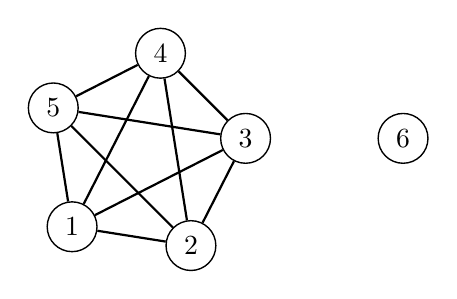
\begin{tikzpicture}
    \GraphInit[vstyle=Normal]\SetGraphUnit{1.3}
    \begin{scope}[rotate=-135]
      \Vertices{circle}{1, 2, 3, 4, 5}
    \end{scope}
    \EA[unit= 2](3){6}
    \Edges(1, 2, 3, 4, 5, 1, 3, 5)
    \Edges(1, 4, 2, 5)
    \end{tikzpicture}
\end{center}
\end{frame}
%typo revised, Compnents -> Components -14p KSS-
\begin{frame}[t]
  \frametitle{Connectedness}
There are two types of connected components in digraphs
\begin{itemize}
\item Strong Components
  \begin{itemize}
  \item maximal subgraph in which there is a path from every vertex to every vertex following all the edges in the direction they are pointing
  \end{itemize}
\item Weak Components
  \begin{itemize}
  \item maximal subgraph which would be connected if we ignore the direction of the edges
  \end{itemize}
\end{itemize}

\end{frame}

\begin{frame}[t]
  \frametitle{Cycles and Connectedness}
Removal of an edge that is on a cycle does not affect connectedness
\begin{center}
    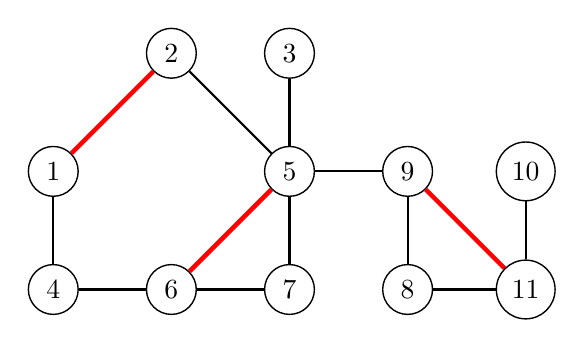
\begin{tikzpicture}
    \GraphInit[vstyle=Normal]\SetGraphUnit{1.5}
    \Vertex{1}
    \NOEA(1){2}
    \SOEA(2){5}
    \NO(5){3}
    \SO(1){4}
    \EA(4){6}
    \EA(6){7}
    \EA(5){9}
    \SO(9){8}
    \SOEA(9){11}
    \EA(9){10}

    \Edges(1, 2, 5, 3)
    \Edges(1, 4, 6, 7, 5)
    \Edges(5, 9, 8, 11, 10)

    \SetUpEdge[style={ultra thick}, color=red]
    \Edges(5, 6)
    \Edges(1, 2)
    \Edges(9, 11)
    \end{tikzpicture}
\end{center}
\end{frame}

\begin{frame}[t]
  \frametitle{Cycles and Connectedness}
Connected subgraph with all vertices and minimum number of edges hs no cycles
\begin{center}
    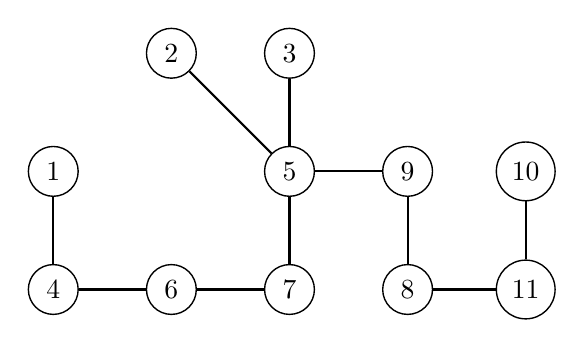
\begin{tikzpicture}
    \GraphInit[vstyle=Normal]\SetGraphUnit{1.5}
    \Vertex{1}
    \NOEA(1){2}
    \SOEA(2){5}
    \NO(5){3}
    \SO(1){4}
    \EA(4){6}
    \EA(6){7}
    \EA(5){9}
    \SO(9){8}
    \SOEA(9){11}
    \EA(9){10}

    \Edges(2, 5, 3)
    \Edges(1, 4, 6, 7, 5)
    \Edges(5, 9, 8, 11, 10)

    \end{tikzpicture}
\end{center}
\end{frame}


\begin{frame}[t]
  \frametitle{Tree}
A tree can be thought of as connected graph that has no cycles
\begin{itemize}
\item $n$ vertex connected graph with $n-1$ edges
\end{itemize}
\end{frame}





\subsection{Spanning Tree}
\begin{frame}[t]
  \frametitle{Spanning Tree}
  \begin{itemize}
  \item Subgraph that includes all vertices of the original graph.
  \item Subgraph is a tree.
    \begin{itemize}
    \item If original graph has $n$ vertices, the spanning tree has $n$
      vertices and $n-1$ edges.
    \end{itemize}

  \end{itemize}

\end{frame}


\begin{frame}[t]
%add additional word -20p KSS-
  \frametitle{Minimum Cost Spanning Tree : MST}
  \begin{itemize}
  \item Tree cost is sum of edge weights/costs
  \end{itemize}
\begin{center}
    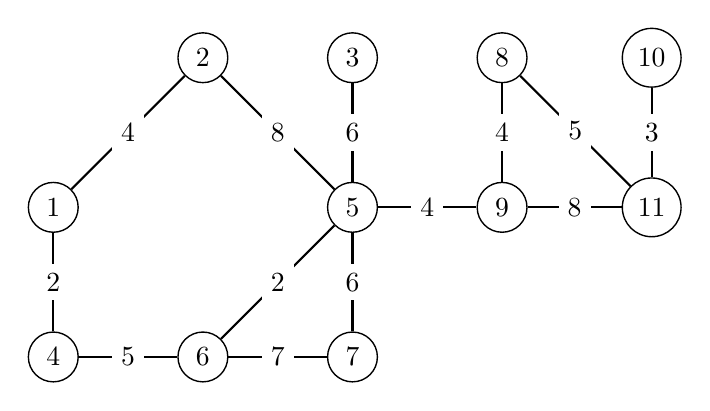
\begin{tikzpicture}
    \GraphInit[vstyle=Normal]\SetGraphUnit{1.9}
    \Vertex{1}
    \NOEA(1){2}
    \SOEA(2){5}
    \NO(5){3}
    \SO(1){4}
    \EA(4){6}
    \EA(6){7}
    \EA(5){9}
    \NO(9){8}
    \NOEA(9){10}
    \EA(9){11}

    \Edges[label=2](1, 4)
    \Edges[label=5](4, 6)
    \Edges[label=2](6, 5)
    \Edges[label=7](6, 7)
    \Edges[label=6](7, 5)
    \Edges[label=4](1, 2)
    \Edges[label=8](2, 5)
    \Edges[label=6](5, 3)
    \Edges[label=4](5, 9)
    \Edges[label=4](9, 8)
    \Edges[label=8](9, 11)
    \Edges[label=5](8, 11)
    \Edges[label=3](11, 10)
    \end{tikzpicture}
\end{center}

\end{frame}


\begin{frame}[t]
  \frametitle{A Spanning Tree}
  \begin{itemize}
  \item Spanning Tree cost is 51
  \end{itemize}
\begin{center}
    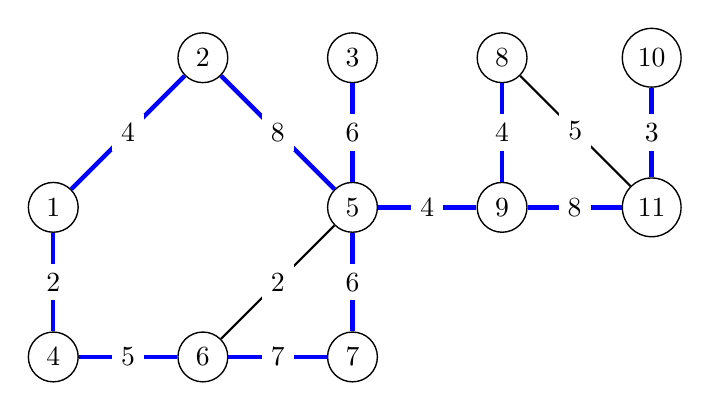
\begin{tikzpicture}
    \GraphInit[vstyle=Normal]\SetGraphUnit{1.9}
    \Vertex{1}
    \NOEA(1){2}
    \SOEA(2){5}
    \NO(5){3}
    \SO(1){4}
    \EA(4){6}
    \EA(6){7}
    \EA(5){9}
    \NO(9){8}
    \NOEA(9){10}
    \EA(9){11}

    \Edges[label=2](6, 5)
    \Edges[label=5](8, 11)

    \SetUpEdge[style={ultra thick}, color=blue]
    \Edges[label=2](1, 4)
    \Edges[label=5](4, 6)
    \Edges[label=7](6, 7)
    \Edges[label=6](7, 5)
    \Edges[label=4](1, 2)
    \Edges[label=8](2, 5)
    \Edges[label=6](5, 3)
    \Edges[label=4](5, 9)
    \Edges[label=4](9, 8)
    \Edges[label=8](9, 11)
    \Edges[label=3](11, 10)
    \end{tikzpicture}
\end{center}

\end{frame}

\begin{frame}[t]
  \frametitle{A Spanning Tree}
  %add additional discription -22p KSS-
  \begin{itemize}
  \item Spanning Tree cost is 41 (= MST)
  \end{itemize}
\begin{center}
    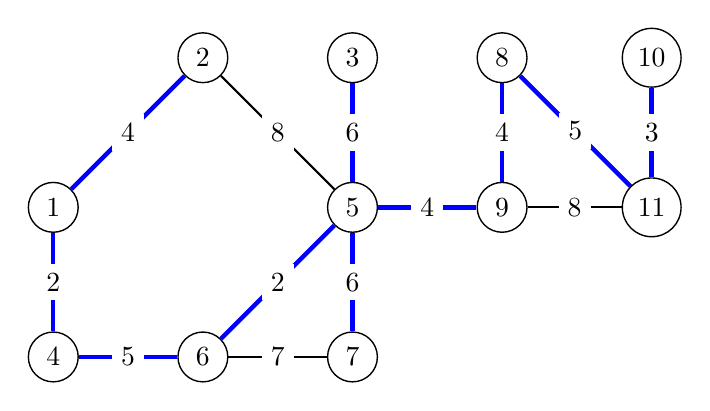
\begin{tikzpicture}
    \GraphInit[vstyle=Normal]\SetGraphUnit{1.9}
    \Vertex{1}
    \NOEA(1){2}
    \SOEA(2){5}
    \NO(5){3}
    \SO(1){4}
    \EA(4){6}
    \EA(6){7}
    \EA(5){9}
    \NO(9){8}
    \NOEA(9){10}
    \EA(9){11}

    \Edges[label=8](2, 5)
    \Edges[label=7](6, 7)
    \Edges[label=8](9, 11)

    \SetUpEdge[style={ultra thick}, color=blue]
    \Edges[label=2](1, 4)
    \Edges[label=5](4, 6)
    \Edges[label=6](7, 5)
    \Edges[label=4](1, 2)
    \Edges[label=2](6, 5)
    \Edges[label=6](5, 3)
    \Edges[label=4](5, 9)
    \Edges[label=4](9, 8)
    \Edges[label=5](8, 11)
    \Edges[label=3](11, 10)
    \end{tikzpicture}
\end{center}

\end{frame}



\begin{frame}[t]
  \frametitle{Minimum-Cost Spanning Tree}
  \begin{itemize}
  \item Weighted connected undirected graph
  \item Spanning tree
  \item Cost of spanning tree is sum of edge costs
  \item Find spanning tree that has minimum cost
  \end{itemize}
\end{frame}


\begin{frame}[t]
  \frametitle{Example}
  %add question for MST -24p KSS-
  \begin{itemize}
  \item Network has 10 edges
  \item Spanning tree has only $n-1 =7 $ edges
  \item Need to either select 7 edges or discard 3
  \item Which edges should be discarded to become MST ?
  \end{itemize}
\begin{center}
    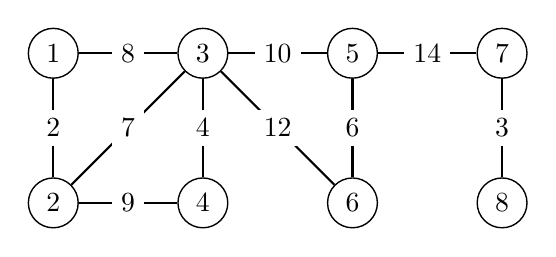
\begin{tikzpicture}
    \GraphInit[vstyle=Normal]\SetGraphUnit{1.9}
    \Vertex{1}
    \SO(1){2}
    \EA(1){3}
    \SOEA(1){4}
    \EA(3){5}
    \SOEA(3){6}
    \EA(5){7}
    \SOEA(5){8}

    \Edges[label=2](1, 2)
    \Edges[label=8](1, 3)
    \Edges[label=7](2, 3)
    \Edges[label=9](2, 4)
    \Edges[label=4](3, 4)
    \Edges[label=10](3, 5)
    \Edges[label=12](3, 6)
    \Edges[label=6](5, 6)
    \Edges[label=14](5, 7)
    \Edges[label=3](7, 8)
    \end{tikzpicture}
\end{center}

\end{frame}

\begin{frame}[t]
	\frametitle{Example : Answer}
	%add question for MST -25p KSS-
	\begin{itemize}
		\item Which edges should be discarded to become MST ?
	\end{itemize}
\begin{center}
		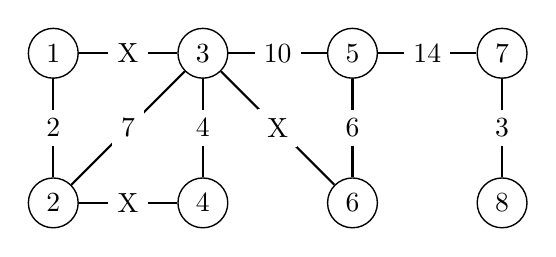
\begin{tikzpicture}
		\GraphInit[vstyle=Normal]\SetGraphUnit{1.9}
		\Vertex{1}
		\SO(1){2}
		\EA(1){3}
		\SOEA(1){4}
		\EA(3){5}
		\SOEA(3){6}
		\EA(5){7}
		\SOEA(5){8}
		
		\Edges[label=2](1, 2)
		\Edges[label=X](1, 3)
		\Edges[label=7](2, 3)
		\Edges[label=X](2, 4)
		\Edges[label=4](3, 4)
		\Edges[label=10](3, 5)
		\Edges[label=X](3, 6)
		\Edges[label=6](5, 6)
		\Edges[label=14](5, 7)
		\Edges[label=3](7, 8)
		\end{tikzpicture}
	
\end{center}
\end{frame}

\begin{frame}[t]
	\frametitle{Example : Answer}
	%add question for MST -26p KSS-
	\begin{itemize}
		\item Which edges should be discarded to become MST ?
	\end{itemize}
	\begin{center}
		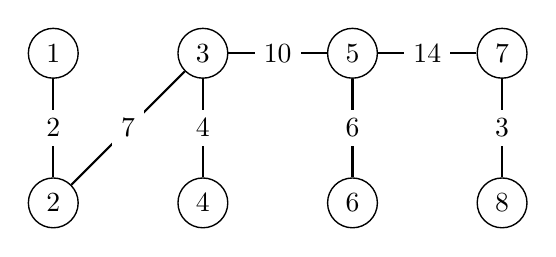
\begin{tikzpicture}
		\GraphInit[vstyle=Normal]\SetGraphUnit{1.9}
		\Vertex{1}
		\SO(1){2}
		\EA(1){3}
		\SOEA(1){4}
		\EA(3){5}
		\SOEA(3){6}
		\EA(5){7}
		\SOEA(5){8}
		
		\Edges[label=2](1, 2)
		\Edges[label=7](2, 3)
		\Edges[label=4](3, 4)
		\Edges[label=10](3, 5)
		\Edges[label=6](5, 6)
		\Edges[label=14](5, 7)
		\Edges[label=3](7, 8)
		\end{tikzpicture}
	\end{center}
\end{frame}

\subsection{Greedy Strategy}
\begin{frame}[t]
  \frametitle{Edge Selection Greedy Strategies}
  \begin{itemize}
  \item Start with an $n-vertex$, $0-edge$ forest. Consider edges in ascending order of cost. Select edge if it does not form a cycle together with already selected edges.
    \begin{itemize}
    \item Kruskal's algorithm
    \end{itemize}

\item Start with a $1-vertex$ tree and grow it into an $n-vertex$ tree by repeatedly adding a vertex and an edge. When there is a choice, add a least cost edge.
  \begin{itemize}
  \item Prim's algorithm
  \end{itemize}
\item Start with an $n-vertex$ forest. Each component/tree selects a least cost edge to connect to another component/tree. Eliminate duplicate selections and possible cycles. Repeat until only 1 component/tree is left.
  \begin{itemize}
  \item Sollin's algorithm
  \end{itemize}

  \end{itemize}
\end{frame}


\begin{frame}[t]
  \frametitle{Edge Rejection Greedy Strategies}
  \begin{itemize}
  \item Start with the connected graph. Repeatedly find a cycle and eliminate the highest cost edge on this cycle. Stop when no cycles remain.
  \item Consider edges in descending order of cost. Eliminate an edge provided this leaves behind a connected graph.
  \end{itemize}
\end{frame}

\subsection{Kruskal's Algorithm}
\begin{frame}[t]
  \frametitle{Kruskal's Algorithm}
\begin{itemize}
  \item Start with a forest that has no edges
  \item  Consider edges in ascending order of cost.
  \item<2-> Edge $(1,2)$ is considered first and added to the forest.
\end{itemize}

{\footnotesize
\begin{columns}
\column{0.19\textwidth}
    \begin{itemize}
\item<3-> Edge $(7,8)$
\item<6-> Edge $(2,3)$
\item<9-> Edge $(3,5)$
    \end{itemize}

\column{0.47\textwidth}
    \begin{itemize}
\item<4-> Edge $(3,4)$
\item<7-> Edge $(1,3)$ creates cycle (\texttt{rejected})
\item<10-> Edge $(3,6)$  creates cycle
    \end{itemize}    

\column{0.39\textwidth}
    \begin{itemize}
\item<5-> Edge $(5,6)$
\item<8-> Edge $(2,4)$  creates cycle
\item<11-> Edge $(5,7)$
    \end{itemize}    
\end{columns}}

\begin{columns}
  \begin{column}{0.5\textwidth}
\begin{center}
    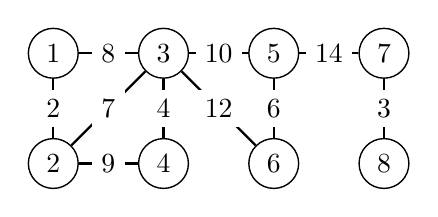
\begin{tikzpicture}
    \GraphInit[vstyle=Normal]\SetGraphUnit{1.4}
    \Vertex{1}
    \SO(1){2}
    \EA(1){3}
    \SOEA(1){4}
    \EA(3){5}
    \SOEA(3){6}
    \EA(5){7}
    \SOEA(5){8}

    \Edges[label=2](1, 2)
    \Edges[label=8](1, 3)
    \Edges[label=7](2, 3)
    \Edges[label=9](2, 4)
    \Edges[label=4](3, 4)
    \Edges[label=10](3, 5)
    \Edges[label=12](3, 6)
    \Edges[label=6](5, 6)
    \Edges[label=14](5, 7)
    \Edges[label=3](7, 8)
    \end{tikzpicture}
\end{center}    
  \end{column}
  \begin{column}{0.5\textwidth}
\begin{center}
    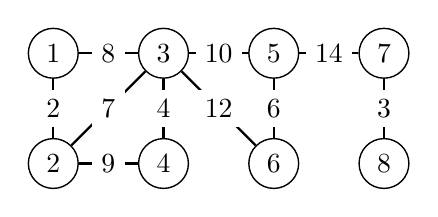
\begin{tikzpicture}
    \GraphInit[vstyle=Normal]\SetGraphUnit{1.4}
    \Vertex{1}
    \SO(1){2}
    \EA(1){3}
    \SOEA(1){4}
    \EA(3){5}
    \SOEA(3){6}
    \EA(5){7}
    \SOEA(5){8}

    \visible<2->{\Edges[label=2](1, 2)}
    \visible<7-7>{\Edges[label=8](1, 3)}
    \visible<6->{\Edges[label=7](2, 3)}
    \visible<8-8>{\Edges[label=9](2, 4)}
    \visible<4->{\Edges[label=4](3, 4)}
    \visible<9->{\Edges[label=10](3, 5)}
    \visible<10-10>{\Edges[label=12](3, 6)}
    \visible<5->{\Edges[label=6](5, 6)}
    \visible<11->{\Edges[label=14](5, 7)}
    \visible<3->{\Edges[label=3](7, 8)}
    \end{tikzpicture}
\end{center}        
  \end{column}
\end{columns}
\end{frame}


\begin{frame}[t]
  \frametitle{Kruskal's Algorithm}
  \begin{itemize}
  \item $n-1$ edges have been selected and no cycle formed, so we must have a spanning tree
    \begin{itemize}
    \item The cost is 46
    \end{itemize}
   \item The minimum cost spanning tree is unique when all edge costs are different
  \end{itemize}
\begin{columns}
  \begin{column}{0.5\textwidth}
\begin{center}
    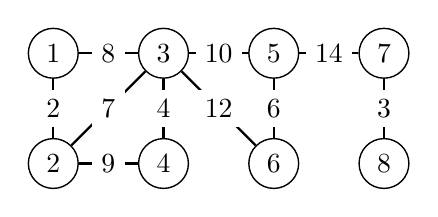
\begin{tikzpicture}
    \GraphInit[vstyle=Normal]\SetGraphUnit{1.4}
    \Vertex{1}
    \SO(1){2}
    \EA(1){3}
    \SOEA(1){4}
    \EA(3){5}
    \SOEA(3){6}
    \EA(5){7}
    \SOEA(5){8}

    \Edges[label=2](1, 2)
    \Edges[label=8](1, 3)
    \Edges[label=7](2, 3)
    \Edges[label=9](2, 4)
    \Edges[label=4](3, 4)
    \Edges[label=10](3, 5)
    \Edges[label=12](3, 6)
    \Edges[label=6](5, 6)
    \Edges[label=14](5, 7)
    \Edges[label=3](7, 8)
    \end{tikzpicture}
\end{center}    
  \end{column}
  \begin{column}{0.5\textwidth}
\begin{center}
    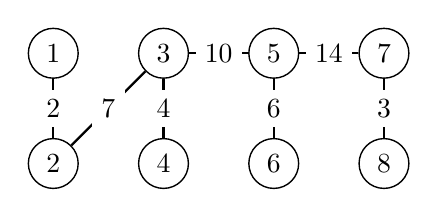
\begin{tikzpicture}
    \GraphInit[vstyle=Normal]\SetGraphUnit{1.4}
    \Vertex{1}
    \SO(1){2}
    \EA(1){3}
    \SOEA(1){4}
    \EA(3){5}
    \SOEA(3){6}
    \EA(5){7}
    \SOEA(5){8}

    \Edges[label=2](1, 2)
    \Edges[label=7](2, 3)
    \Edges[label=4](3, 4)
    \Edges[label=10](3, 5)
    \Edges[label=6](5, 6)
    \Edges[label=14](5, 7)
    \Edges[label=3](7, 8)
    \end{tikzpicture}
\end{center}        
  \end{column}
\end{columns}
\end{frame}


\begin{frame}[t]
  \frametitle{Prim's Algorithm}
  \begin{itemize}
  \item Start with any single vertex tree
  \item Get a 2-vertex tree by adding a cheapest edge
  \item Get a 3-vertex tree by adding a cheapest edge
  \item Grow the tree one edge at a time until the tree has $n-1$ edges (and hence has all n vertices)
  \end{itemize}

\begin{columns}
  \begin{column}{0.5\textwidth}
\begin{center}
    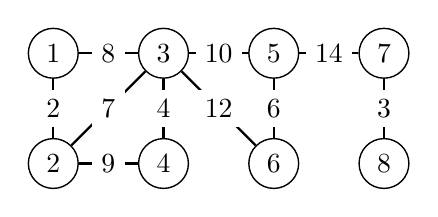
\begin{tikzpicture}
    \GraphInit[vstyle=Normal]\SetGraphUnit{1.4}
    \Vertex{1}
    \SO(1){2}
    \EA(1){3}
    \SOEA(1){4}
    \EA(3){5}
    \SOEA(3){6}
    \EA(5){7}
    \SOEA(5){8}

    \Edges[label=2](1, 2)
    \Edges[label=8](1, 3)
    \Edges[label=7](2, 3)
    \Edges[label=9](2, 4)
    \Edges[label=4](3, 4)
    \Edges[label=10](3, 5)
    \Edges[label=12](3, 6)
    \Edges[label=6](5, 6)
    \Edges[label=14](5, 7)
    \Edges[label=3](7, 8)
    \end{tikzpicture}
\end{center}    
  \end{column}
  \begin{column}{0.5\textwidth}
\begin{center}
    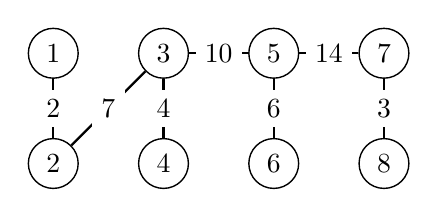
\begin{tikzpicture}
    \GraphInit[vstyle=Normal]\SetGraphUnit{1.4}
    \Vertex{1}
    \SO(1){2}
    \EA(1){3}
    \SOEA(1){4}
    \EA(3){5}
    \SOEA(3){6}
    \EA(5){7}
    \SOEA(5){8}

    \visible<2->{\Edges[label=2](1, 2)}
    \visible<3->{\Edges[label=7](2, 3)}
    \visible<4->{\Edges[label=4](3, 4)}
    \visible<5->{\Edges[label=10](3, 5)}
    \visible<6->{\Edges[label=6](5, 6)}
    \visible<7->{\Edges[label=14](5, 7)}
    \visible<8->{\Edges[label=3](7, 8)}
    \end{tikzpicture}
\end{center}        
  \end{column}
\end{columns}

\end{frame}


\begin{frame}[t]
  \frametitle{Sollin's Algorithm}
  \begin{itemize}
  \item Start with a forest that has no edges.
  \item Each component selects a least cost edge with which to connect
    to another component.
  \item Duplicate selections are eliminated.
  \item Cycles are possible when the graph has some edges that have
    the same cost.
  \item Each component that remains selects a least cost edge with which to connect to another component. 
  \item Beware of duplicate selections and cycles.
  \end{itemize}
\begin{columns}
  \begin{column}{0.5\textwidth}
\begin{center}
    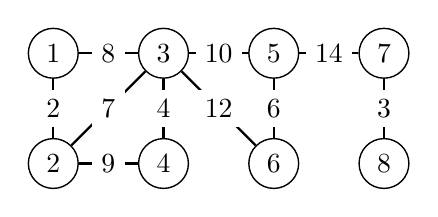
\begin{tikzpicture}
    \GraphInit[vstyle=Normal]\SetGraphUnit{1.4}
    \Vertex{1}
    \SO(1){2}
    \EA(1){3}
    \SOEA(1){4}
    \EA(3){5}
    \SOEA(3){6}
    \EA(5){7}
    \SOEA(5){8}

    \Edges[label=2](1, 2)
    \Edges[label=8](1, 3)
    \Edges[label=7](2, 3)
    \Edges[label=9](2, 4)
    \Edges[label=4](3, 4)
    \Edges[label=10](3, 5)
    \Edges[label=12](3, 6)
    \Edges[label=6](5, 6)
    \Edges[label=14](5, 7)
    \Edges[label=3](7, 8)
    \end{tikzpicture}
\end{center}    
  \end{column}
  \begin{column}{0.5\textwidth}
\begin{center}
    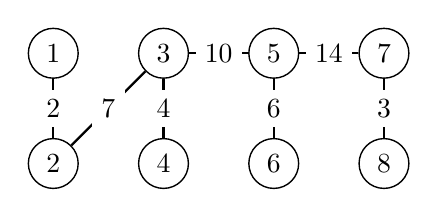
\begin{tikzpicture}
    \GraphInit[vstyle=Normal]\SetGraphUnit{1.4}
    \Vertex{1}
    \SO(1){2}
    \EA(1){3}
    \SOEA(1){4}
    \EA(3){5}
    \SOEA(3){6}
    \EA(5){7}
    \SOEA(5){8}

    \visible<2->{\Edges[label=2](1, 2)}
    \visible<3->{\Edges[label=7](2, 3)}
    \visible<2->{\Edges[label=4](3, 4)}
    \visible<3->{\Edges[label=10](3, 5)}
    \visible<2->{\Edges[label=6](5, 6)}
    \visible<3->{\Edges[label=14](5, 7)}
    \visible<2->{\Edges[label=3](7, 8)}
    \end{tikzpicture}
\end{center}        
  \end{column}
\end{columns}

\end{frame}


\begin{frame}[t]
  \frametitle{Greedy Minimum-Cost Spanning Tree Algorithms}
  \begin{itemize}
  \item Can prove that all result in a minimum-cost spanning tree.
  \item Prim's Algorithm is the fastest
    \begin{itemize}
    \item $O(n^2)$ using an implementation similar to that of Dijkstra's shortest-path algorithm
    \item $O(e+n\log n)$ using a Fibonacci heap
    \end{itemize}
  \item Kruskal's algorithm uses \textbf{union-find trees} to run in $O(n+e \log e)$ time
    \begin{itemize}
    \item \texttt{union(x,y)} joins two subsets containing \texttt{x} and \texttt{y} into a single subset
    \item \texttt{find(x)} determines the subset with the element \texttt{x}
    \end{itemize}
  \end{itemize}
\end{frame}


\begin{frame}[t]
  \frametitle{Exmple: Union-find}
Assume the following set $S=\{1, 2, 3, 4, 5, 6\}$ and create a six independent sets: $\{1\}, \{2\}, \{3\}, \{4\}, \{5\}, \{6\}$.

After performing \texttt{union(1, 4)} and \texttt{union(2, 5)}, then we have $\{1, 4\}, \{5, 2\}, \{3\}, \{4\}$

After running \texttt{union(2, 1)} and \texttt{union(3, 6)}, then we have $\{1, 2, 4, 5\}, \{3, 6\}$


\begin{columns}
\column{0.5\textwidth}
    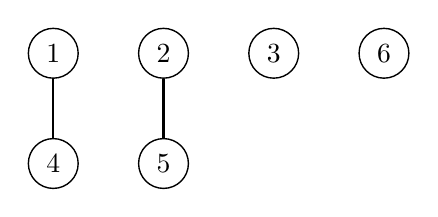
\begin{tikzpicture}
    \GraphInit[vstyle=Normal]\SetGraphUnit{1.4}
    \Vertex{1}
    \SO(1){4}
    \EA(1){2}
    \SO(2){5}
    \EA(2){3}
    \EA(3){6}
    \Edges(1, 4)
    \Edges(2, 5)
    \end{tikzpicture}
\column{0.5\textwidth}
    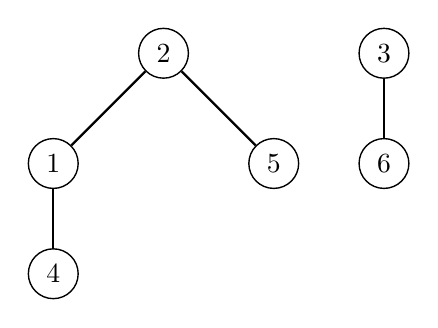
\begin{tikzpicture}
    \GraphInit[vstyle=Normal]\SetGraphUnit{1.4}
    \Vertex{2}
    \SOWE(2){1}
    \SOEA(2){5}
    \SO(1){4}
    \EA(5){6}
    \NO(6){3}
    \Edges(2, 1)
    \Edges(2, 5)
    \Edges(1, 4)
    \Edges(3, 6)
    \end{tikzpicture}
\end{columns}
\end{frame}

\begin{comment}
\begin{frame}[t]
  \frametitle{The code: union-find}

\end{frame}


\begin{frame}[t]
  \frametitle{}
\end{frame}
\end{comment}

\end{document}
